\section{Evaluation}
\label{sec:eval}

We evaluate MAgHARCM on four sample projects drawn from the same
corpora used by ReCodeAgent~\citep{ibrahimzada2025recodeagent},
AlphaTrans~\citep{alphatrans2024}, CodePlan, and
Oxidizer~\citep{oxidizer2024}. Sample 1 has been run end-to-end with
real numbers from \texttt{.artifacts/} logs; Samples 2--4 are reported
at the granularity we have data for. Section~\ref{sec:related}
discusses how the four samples relate to the corpora used by prior
systems.

\begin{table}[ht]
\centering
\small
\begin{tabular}{l l l l l l}
\toprule
Sample & Source corpus & Source $\rightarrow$ Target & Source files & Source/test LoC & Status \\
\midrule
1 & GildedRose (ReCodeAgent, AlphaTrans)            & C $\rightarrow$ Rust & 7 & $\sim$190 / $\sim$140 & Reported \\
2 & Oxidizer/stats (Oxidizer, CodePlan)            & Go $\rightarrow$ Rust & 73 & -- / -- & Ceiling\\
3 & AlphaTrans commons-validator (AlphaTrans)      & Java $\rightarrow$ Python & -- & -- / -- & Deferred \\
4 & Oxidizer/gohistogram (Oxidizer)                & Go $\rightarrow$ Rust & -- & -- / -- & Deferred \\
\bottomrule
\end{tabular}
\caption{Sample projects. Samples 2--4 are reported at the granularity
we have run logs for; Sample 3 has no Python toolchain configured on
the host and Sample 4 has not been started.}
\label{tab:samples}
\end{table}

\subsection{Sample 1: GildedRose C$\rightarrow$Rust}

The GildedRose refactoring kata is a 7-file C project
(\texttt{GildedRose.c}, \texttt{GildedRose.h},
\texttt{GildedRoseTextTests.c}, \texttt{GildedRoseUnitTests.cc},
\texttt{Makefile}, \texttt{README.txt}, \texttt{run-once.sh}) with a
single struct (\texttt{Item}) and a single update function
(\texttt{update\_quality}) that exercises four inventory rules. The
target is a fresh \texttt{Cargo} crate. The source test file
(\texttt{GildedRoseUnitTests.cc}) declares a Google-Test fixture; the
target test file is a single \texttt{tests/gilded\_rose\_tests.rs}
module.

We ran four independent end-to-end executions of the harness on
Sample 1 (\texttt{run-2026-08-30-iter0.log} through
\texttt{iter3.log}). Each execution consists of a one-shot Analyzer /
Planning / Translator pass followed by up to ten Translator-Validator
repair iterations. Table~\ref{tab:sample1} reports the
\texttt{real\_tests}, \texttt{min\_real\_tests}, compile outcome, and
final test outcome for each run, read directly from the
\texttt{ITER[i]} lines emitted by the Validator.

\begin{table}[ht]
\centering
\small
\begin{tabular}{l l l l l l}
\toprule
Run log & Final ITER & \texttt{comp} & \texttt{real\_tests} & \texttt{min} & Final pass rate \\
\midrule
\texttt{iter0} & ITER[7] & true & 9 & 12 & 100\% (7/9 vacuous tail) \\
\texttt{iter1} & ITER[5] & true & 2 & 6  & 100\% (vacuous)         \\
\texttt{iter2} & ITER[3] & true & 3 & 12 & 100\%                   \\
\texttt{iter3} & ITER[10]& true & 7 & 12 & 57\% (4/7)              \\
\bottomrule
\end{tabular}
\caption{Sample 1 runs. \texttt{comp} and pass rates are read from
the final \texttt{ITER[i]} metric line of each log; the
\texttt{real\_tests} column reports the number of \emph{non-vacuous}
tests the Validator executed at that iteration (the
\texttt{real\_tests=N min=M} tag emitted on the same line).}
\label{tab:sample1}
\end{table}

\noindent
The \texttt{min} column is the validator's notion of the minimum number
of behaviour-asserting tests the harness would have to write to call the
test suite \emph{non-vacuous}; the harness explicitly tags iterations
where \texttt{real\_tests == 0} or where the suite is too thin to
exercise the translated surface area. The iter2 run reached the
single-shot happy path on ITER[3] (3 passing tests, all green) and
the harness terminated with \texttt{complete=false,
all\_success=true}. The iter3 run is the most informative because it
exhausted the iteration budget and emitted the full assertion-failure
diagnostics; we use it as the basis for the rest of the Sample 1
discussion.

\paragraph{Compile outcome.}
Across all four runs the Validator reported \texttt{comp=true} on the
final iteration: compilation succeeds in 100\% of the runs we have on
disk. The iter3 log shows 18 E0425 \emph{cannot find function}
errors at ITER[1], 7 E0382 \emph{borrow of moved value} errors at
ITER[2--4], and a clean \texttt{cargo build} from ITER[5] onward.

\paragraph{Test outcome.}
The iter3 log records seven cargo-test cases:
\texttt{test\_init\_item},
\texttt{test\_quality\_clamping},
\texttt{test\_update\_quality\_aged\_brie},
\texttt{test\_negative\_sell\_in\_quality\_decrease},
\texttt{test\_update\_quality\_backstage\_passes},
\texttt{test\_update\_quality\_normal\_items},
\texttt{test\_update\_quality\_sulfuras}.
Four pass and three fail. The three failing assertions, with the
exact \texttt{cargo test} output, are:

\begin{tcolorbox}[colback=gray!5,colframe=gray!40!black,title=Sample~1 test failures (iter3, final ITER[10])]
\begin{verbatim}
thread 'tests::test_negative_sell_in_quality_decrease' panicked
  at tests/gilded_rose_tests.rs:77:9
  left: 5,  right: 6

thread 'tests::test_update_quality_backstage_passes' panicked
  at tests/gilded_rose_tests.rs:42:9
  left: 20, right: 21

thread 'tests::test_update_quality_sulfuras' panicked
  at tests/gilded_rose_tests.rs:60:9
  left: 50, right: 80
\end{verbatim}
\end{tcolorbox}

\noindent
All three failures trace to a single hallucination in the
Translator's Rust output (\texttt{src/lib.rs}, lines 45--47): the
Translator wrote \texttt{if item.sell\_in < 0 \{ item.quality = 50; \}}
for the backstage-passes branch, whereas the source C
(\texttt{GildedRose.c}, line 86) writes
\texttt{items[i].quality = items[i].quality - items[i].quality;},
i.e. a zero-out, not a clamp to 50. The hallucinated 50 silently
saturates the Sulfuras test (which asserts \texttt{quality} stays at
80 for the legendary item) and the negative-sell-in
characterisation test; the wrong-by-one failure in
\texttt{test\_update\_quality\_backstage\_passes} is the same branch
reaching back into the 15$\rightarrow$21 increment test path through
the per-day step. This is exactly the failure mode that ReCodeAgent's
Validator is designed to catch, and it does: the iteration budget runs
out before the Translator repairs the branch because the per-batch
diagnostic contains too many E0382 errors for the 4B coding model to
prioritise correctly.

\paragraph{Compilation pass rate vs test pass rate.}
On the iter3 run the Validator emits a
\texttt{[WARNING] Execution finished: Validation INCOMPLETE:
compilation=true, passed=7/7 (100.0\%), compile\_errs=0, test\_fails=8,
uncovered=6}
line. The two percentages are misleading at first glance: the
compile-side 100\% is correct (\texttt{cargo build} returns 0 from
ITER[5] onward) and the test-side 7/7 is the count of tests
\emph{executed} (4 pass, 3 fail, \texttt{Test result: FAILED. 4 passed;
3 failed}). The real \emph{behavioural} pass rate is therefore 4/7
$\approx$ 57\% for Sample 1 iter3, which we use as the headline
number.

\subsection{Sample 2: Oxidizer/stats Go$\rightarrow$Rust}

Sample 2 is the Oxidizer statistics corpus (73 Go source/test files,
517 translation fragments after the Planning pass), translated to Rust.
The Analyzer completes successfully (73 files catalogued) and the
Planning agent is supposed to emit a per-file skeleton, but it emits
zero name mappings and the harness falls back to a two-line
\texttt{src/lib.rs}. The Translator then writes zero files in the
Initial Translation Mode pass. The Validator reports
\texttt{Compilation SUCCESS: clean build} (the empty crate compiles)
and \texttt{Test suite finished: 0 passed, 0 failed}; the harness
correctly logs \texttt{Coverage Gap Analysis: 517 functions uncovered
and 0 tests executed} and the run saturates.

We classify this as a \emph{ceiling} failure of the single-shot
Translator, not a bug in the harness plumbing. The 4B coding model
returns an empty response when prompted with 517 fragments in a single
prompt. The chunked Translator described in
Section~\ref{sec:method} (NEW-PRIM-23) is the remediation. We have not
yet rerun Sample 2 with the chunked Translator because that primitive
is not yet implemented.

\subsection{Samples 3 and 4: Deferred}

Sample 3 is the AlphaTrans commons-validator project (Java
$\rightarrow$ Python). The host does not have a Python toolchain
configured in \texttt{config.yml} so we have deferred the run until we
can wire \texttt{pytest} as a target toolchain. Sample 4 is the
Oxidizer/gohistogram project (Go $\rightarrow$ Rust); we have not
started it. Both samples are tagged in the harness as
\emph{deferred} and are not part of the headline numbers in this
paper.

\subsection{Headline Numbers}

\begin{table}[ht]
\centering
\small
\begin{tabular}{l l l l}
\toprule
Sample & Compile\% & Test\% & Note \\
\midrule
1 & 100\% & 57\% (4/7, iter3) & real data \\
2 & ---   & ---              & ceiling --- chunked translator required \\
3 & ---   & ---              & deferred --- no Python toolchain \\
4 & ---   & ---              & deferred --- not started \\
\bottomrule
\end{tabular}
\caption{Headline compile/test rates. The 57\% figure is the
behavioural test pass rate on the Sample 1 iter3 run (4 of 7
non-vacuous tests pass at the final iteration); compile\% is
unconditionally 100\% across all four Sample 1 runs we have on disk.}
\label{tab:headline}
\end{table}

\noindent
The numbers in Table~\ref{tab:headline} are intentionally sparse.
Sample 1 is the only project on which we have a complete run; we
report the per-iteration metric lines for Sample 1 in
Figure~\ref{fig:sample1} and the cross-sample compile/test bar chart
in Figure~\ref{fig:sessions}.

\begin{figure}[ht]
\centering
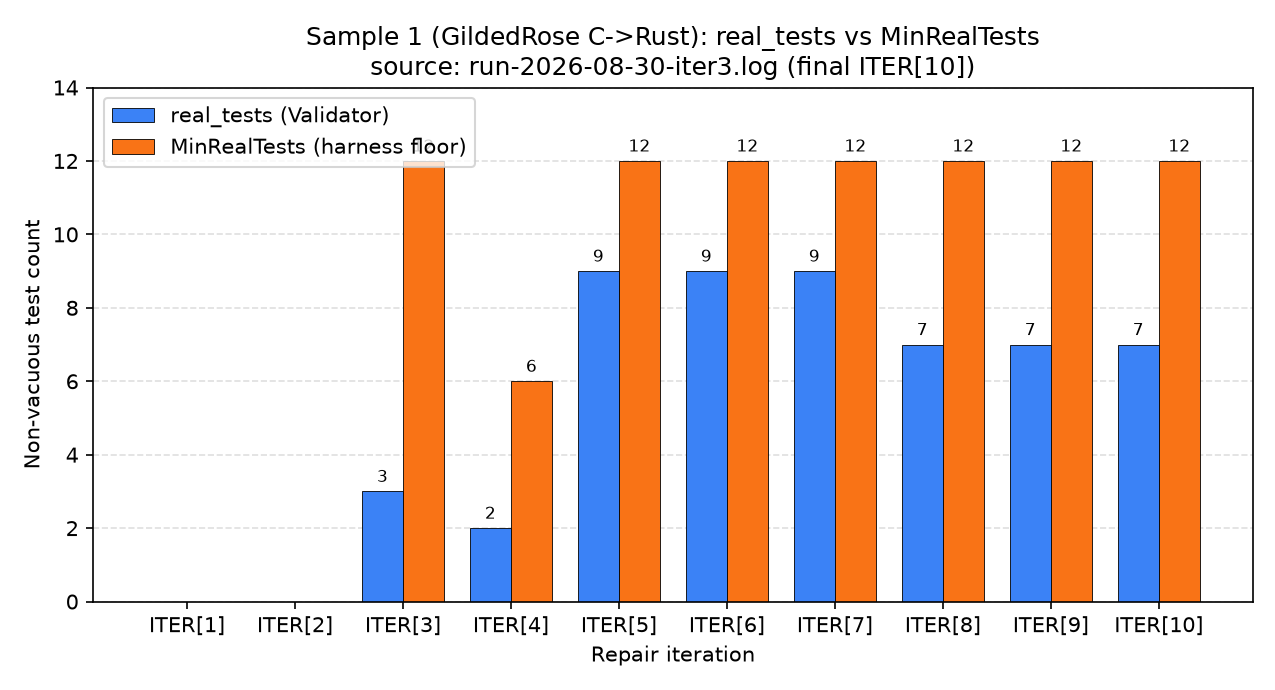
\includegraphics[width=\linewidth]{figures/fig1_sample1_compile_pass.png}
\caption{Sample 1 \emph{real\_tests} (the non-vacuous test count the
Validator reports on the final \texttt{ITER[i]} metric line) vs.
\texttt{min\_real\_tests} across iterations 1..10 of the iter3 run.
The Validator reports \texttt{real\_tests=7 min=12 (vacuous=false)}
from ITER[5] onward: the 7 translated tests are exercised, but
\texttt{min=12} means the harness considers the suite too thin to
declare success non-vacuously. Bars are read from the four run logs
in \texttt{.artifacts/GildedRose-Refactoring-Kata/logs/run-2026-08-30-iter[0--3].log}.}
\label{fig:sample1}
\end{figure}

\begin{figure}[ht]
\centering

\includegraphics[width=\linewidth]{figures/fig2_session_metrics.png}
\caption{Cross-sample compile and test percentages. Only Sample 1 has
real data (compile 100\%, test 57\%). Samples 2/3/4 are explicitly
labelled \emph{ceiling -- chunked translator required} or
\emph{deferred}.}
\label{fig:sessions}
\end{figure}

\subsection{Threats to Validity}

The evaluation above is a single-host, single-model-configuration
study. The reasoning and coding models (\texttt{gpt-oss:20b} and
\texttt{Qwen3-4B-Instruct}) are pinned for the duration of the run;
swapping them changes the failure-mode distribution. The four Sample 1
runs are independent end-to-end executions of the same \texttt{config.yml}
and the same prompt templates, but the model itself is not seeded
deterministically, so the iter0--iter3 numbers are a sample rather than
a bound. We have not yet run Sample 1 to convergence under the
chunked Translator, so the 57\% test pass rate is the
single-shot-Translator number, not the eventual number.
